\documentclass[11pt, a4paper]{article}
\usepackage[english]{babel}
\usepackage[utf8]{inputenc}
\usepackage{fancyhdr}
\usepackage{lastpage}
\usepackage{datetime}
\usepackage{indentfirst}
\usepackage{hyperref}
\usepackage{appendix}
\usepackage{amsmath}
\usepackage{amssymb}
\usepackage{amsfonts}
\usepackage{mathtools}
\usepackage{siunitx}
\usepackage{cancel}
\usepackage{tabularray}
\usepackage{multirow}
\usepackage{array}
\usepackage{hhline}
\usepackage{makecell}
\usepackage{courier}
\usepackage[font=small, skip=0pt]{caption}
\usepackage[font=scriptsize, skip=0pt]{subcaption}
\usepackage{float}
\usepackage{graphicx}
\usepackage{listings}
\usepackage{xcolor}
\usepackage{matlab-prettifier}
\usepackage[T1]{fontenc}
\usepackage{lmodern}
\usepackage{bigfoot}
\usepackage{filecontents}
\usepackage[nottoc]{tocbibind}

\graphicspath{ {./mathimages/} }

\newdateformat{Datea}{\THEDAY\ \monthname[\THEMONTH] \THEYEAR}
\newdateformat{Dateb}{\monthname[\THEMONTH] \THEYEAR}

%\allowdisplaybreaks
\DeclareMathOperator{\cosec}{cosec}
\DeclareMathOperator{\cotan}{cotan}
\DeclareMathOperator{\sech}{sech}
\DeclareMathOperator{\cosech}{cosech}
\DeclareMathOperator{\arcsec}{arcsec}
\DeclareMathOperator{\arccot}{arccot}
\DeclareMathOperator{\arccsc}{arccosec}
\DeclareMathOperator{\arccosh}{arccosh}
\DeclareMathOperator{\arcsinh}{arcsinh}
\DeclareMathOperator{\arctanh}{arctanh}
\DeclareMathOperator{\arcsech}{arcsech}
\DeclareMathOperator{\arccsch}{arccsch}
\DeclareMathOperator{\arccoth}{arccoth}
\DeclareMathOperator{\arsinh}{arsinh}
\DeclareMathOperator{\arcosh}{arcosh}
\DeclareMathOperator{\artanh}{artanh}

\DeclareMathOperator{\cis}{cis}

\pagestyle{fancy}
\fancyhf{}
\rhead{Hatam Barma}
\chead{\begin{tabular}[t]{@{}l@{}}\\Mathematics and Further Mathematics Pure Revision Summary\end{tabular}}
\lhead{\Dateb\today}
\cfoot{Page \thepage}

\renewcommand{\thesection}{\arabic{section}} 

\renewcommand{\thesubsection}{\thesection.\arabic{subsection}}

\setcounter{section}{3}

\allowdisplaybreaks

\fancypagestyle{plain}{
\fancyhf{}
\renewcommand{\headrulewidth}{0pt}}

\hypersetup{
    colorlinks,
    citecolor=black,
    filecolor=black,
    linkcolor=blue,
    urlcolor=magenta!70!black
}

\begin{document}


\begin{titlepage}
   \begin{center}
       \vspace*{2.5cm}
	\huge
       \textbf{A-Level Mathematics and Further Mathematics Pure Revision Summary} \\
	\vspace{1cm}
	\Large
       \textbf{Chapter 4: Trigonometry}
            
       \vspace{1.5cm}
	\LARGE
       \textbf{Hatam Barma} \\
	\vspace{0.75cm}
       \normalsize
       \emph{Compiled on \Datea\today} \\

       \vfill
        

	E-mail: hatam.barma@gmail.com
   \end{center}
\end{titlepage}


\tableofcontents

\clearpage
\section{Trigonometry}
\vspace{0.5cm}


\subsection{Trigonometric values of sin, cos, and tan}
\begin{itemize}
\item A Level M AS / Year 1 \hspace{1cm} \phantom{ } Pages 177 -- 179
\end{itemize} \par
These should all be familiar from GCSE, and while this table is identical to that in section \ref{radianmeasure}, the contents of it remain just as important.
\begin{center}
\begin{tblr}{|[.75pt]|c|c||c|c|c||[.75pt]}
\hline[1.25pt]
$\theta$ in $^{\circ}$ & $\theta$ in radians & $\sin(\theta)$ & $\cos(\theta)$ & $\tan(\theta)$ \\ \hline[.75pt]
$0$ & $0$ & $0$ & $1$ & $0$ \\ \hline
$30$ & $\frac{\pi}{6}$ & $\frac{1}{2}$ & $\frac{\sqrt{3}}{2}$ & $\frac{1}{\sqrt{3}}$ \\ \hline
$45$ & $\frac{\pi}{4}$ & $\frac{1}{\sqrt{2}}$ & $\frac{1}{\sqrt{2}}$ & $1$ \\ \hline
$60$ & $\frac{\pi}{3}$ & $\frac{\sqrt{3}}{2}$ & $\frac{1}{2}$ & $\sqrt{3}$ \\ \hline
$90$ & $\frac{\pi}{2}$ & $1$ & $0$ & $\mathrm{undefined}$ \\ \hline[1pt]
\end{tblr}
\end{center}

\vspace{0.5cm}


\subsection{Sine and cosine rules; area formulae}
\begin{itemize}
\item A Level M AS / Year 1 \hspace{1cm} \phantom{ } Pages 204 -- 217
\end{itemize} \par
These all should be familiar from GCSE;

\begin{table}[H]
\renewcommand{\arraystretch}{1.25}
\begin{tabular}{ll}
Area: & $\frac{ab\sin(C)}{2}=\frac{bc\sin(A)}{2}=\frac{ca\sin(B)}{2}$ \\
Sine rule: & $\frac{a}{\sin(A)}=\frac{b}{\sin(B)}=\frac{c}{\sin(C)}$ \\
Cosine rule: & $a^{2} = b^{2} + c^{2} - 2bc\cos(A)$ \\
\end{tabular}
\end{table}
\vspace{0.5cm}


\subsection{Sine, cosine and the unit circle}
The unit circle is defined by
\begin{equation*}
(x,y)=(\cos(\theta),\sin(\theta))
\end{equation*}
So:
\begin{equation*}
x^{2}+y^{2}=\cos^{2}(\theta)+\sin^{2}(\theta)=1
\end{equation*}
$\tan(\theta)$ gives the gradient of the normal to points on the circle. This can be shown using parametric differentiation (section \ref{parametricdifferentiation})

\vspace{0.5cm}


\subsection{Trigonometric equations, and the Pythagorean identity}
\begin{itemize}
\item A Level M AS / Year 1 \hspace{1cm} \phantom{ } Pages 179 -- 188
\item A Level M Year 2 \hspace{1cm} \phantom{ AS / } Pages 178 -- 182
\end{itemize} \par
We recognise from GCSE the standard trigonometric functions $\sin$, $\cos$ and $\tan$, and that $\tan$ of an angle is defined as the ratio between $\sin$ and $\cos$ $\left(\tan(\theta)\equiv\frac{\sin(\theta)}{\cos(\theta)}\right)$. We can also define the reciprocal trigonometric functions as follows:
\small
\begin{align*}
\cosec(\theta)&=\frac{1}{\sin(\theta)} & \sec(\theta)&=\frac{1}{\cos(\theta)} & \cot(\theta)=\frac{1}{\tan(\theta)}=\frac{\cos(\theta)}{\sin(\theta)}
\end{align*}
\normalsize
We can therefore manipulate the Pythagorean identity,
\begin{equation*}
\sin^{2}(\theta)+\cos^{2}(\theta)\equiv1
\end{equation*}
To give two more identities by dividing through by $\sin^{2}$ or $\cos^{2}$:
\begin{align*}
1+\cot^{2}(\theta)&=\cosec^{2}(\theta) & \tan^{2}(\theta)+1&=\sec^{2}(\theta)
\end{align*}
\normalsize

\vspace{0.5cm}


\subsection{The small-angle approximations}
\begin{itemize}
\item A Level M Year 2 \hspace{1cm} \phantom{ AS / } Pages 155 -- 163
\end{itemize} \par
The small angle approximations for $\sin$, $\cos$, and $\tan$ are as follows:
\begin{figure}[H]
\centering
\begin{subfigure}[b]{0.49\textwidth}
\begin{flalign*}
\sin(\theta)&\approx\theta &&\\
\cos(\theta)&\approx1-\frac{1}{2}\theta^{2} && \\
\tan(\theta)&\approx\theta
\end{flalign*}
\end{subfigure}
\hfill
\begin{subfigure}[b]{0.49\textwidth}
\centering
\scalebox{.85}{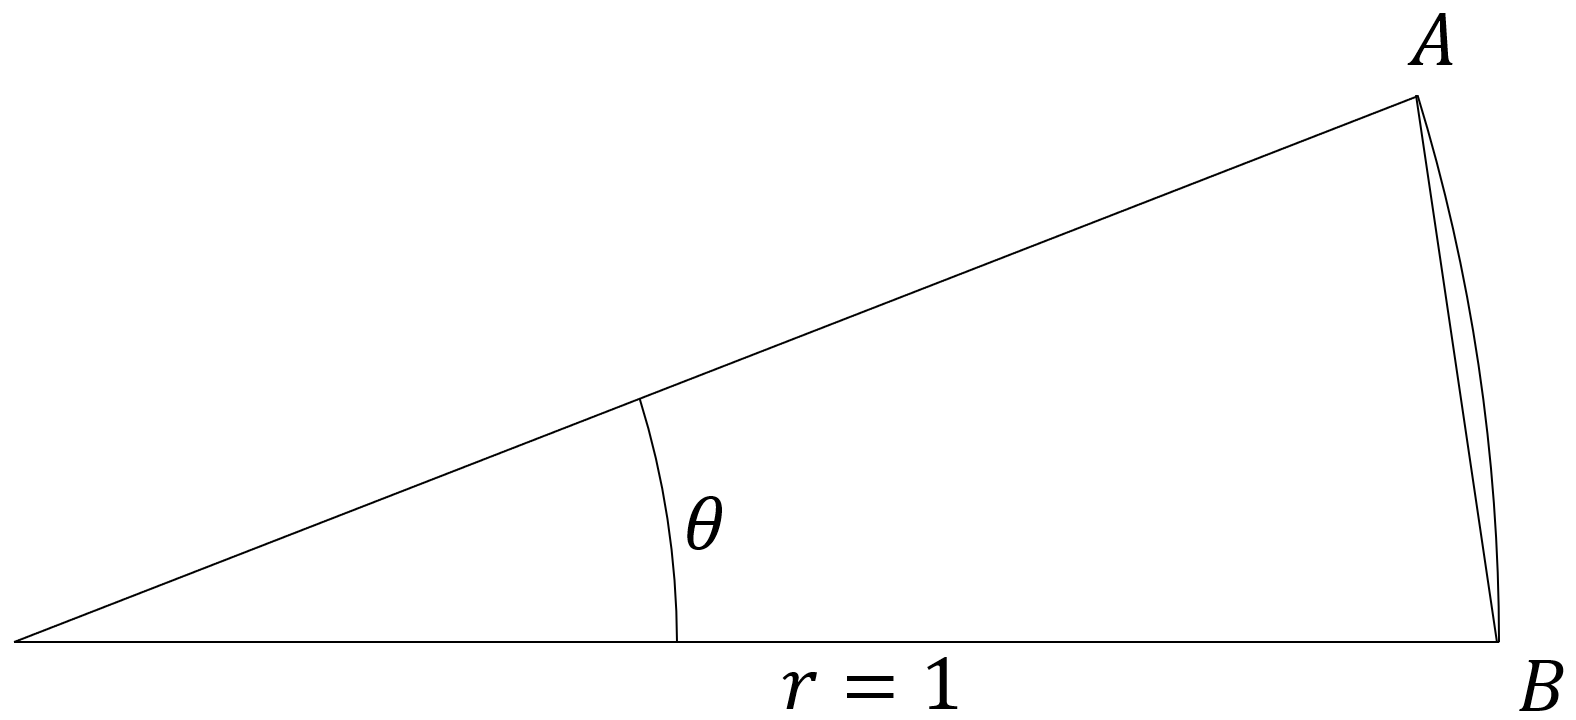
\includegraphics[width=\textwidth]{smallangleapproximation1}}
\end{subfigure}
\end{figure}
\scriptsize
\begin{itemize}
\item[Note:]These are the first terms of the Maclaurin series (see section \ref{standardmaclaurin}) for each of these
\end{itemize}
\normalsize
The arc $AB$ has length $\theta$ (in radians of course), and the chord $AB$ has length $\sin(\theta)$. When $\theta$ is samll:
\begin{flalign*}
AB_{\text{arc}}&\approx AB_{\text{chord}} && \\
\theta&\approx\sin(\theta) &&
\end{flalign*}

We can use a double angle identity (section \ref{doubleangleformulae}) to express $\cos(\theta)$ in terms of $\sin\left(\frac{1}{2}\theta\right)$ terms alone, and thus gain an approximation for $\cos$:
\newpage
\vspace{-.3cm}
\begin{flalign*}
\cos(\theta)&=1-2\sin^{2}\left( \frac{1}{2}\theta \right) && \\
\cos(\theta)&\approx1-2\cdot\left( \frac{1}{2}\theta \right)^{2} && \\
\cos(\theta)&=1-\frac{1}{2}\theta^{2}
\end{flalign*}

Constructing an approximation using this method for $\tan$ requires a little more work, but can still be done relatively easily. First, we assume a quadratic approximation for $\tan(\theta)$, and then substitute in our approximations for $\sin$ and $\cos$ into $\sin(\theta)=\tan(\theta)\cdot\cos(\theta)$:
\begin{flalign*}
\tan(\theta)&\approx p+q\theta+r\theta^{2} && \\
&&&\\
\sin(\theta)&\approx p\cdot\cos(\theta)+q\theta\cdot\cos(\theta)+r\theta^{2}\cdot\cos(\theta) && \\
\theta&\approx p-\frac{p\theta^{2}}{2}+q\theta-\frac{q\theta^{3}}{2}+r\theta^{2}-\frac{r\theta^{4}}{2} && \\
0&\approx p+\theta(q-1)+\theta^{2}(r-\frac{p}{2})+\theta^{3}(-\frac{q}{2})+\theta^{4}(-\frac{r}{2}) &&
\end{flalign*}
Now since we only need terms up to the quadratic;
\begin{flalign*}
p&=0 &&\\
q-1&=0 \hspace{1cm}\Rightarrow \hspace{1cm}q=1 &&\\
r-\frac{p}{2}&=0 \hspace{1cm}\Rightarrow \hspace{1cm}r=0 &&
\end{flalign*}

Therefore;
\begin{flalign*}
\tan(\theta)&\approx0+1\cdot\theta+0\cdot\theta^{2} && \\
\tan(\theta)&\approx\theta &&
\end{flalign*}
\vspace{0.5cm}


\subsection{Double angle formulae}
\label{doubleangleformulae}
\begin{itemize}
\item A Level M Year 2 \hspace{1cm} \phantom{ AS / } Pages 168 -- 173
\end{itemize} \par
A geometric derivation for the double angle formulae for $\sin$, $\cos$, and $\tan$ is provided here. A matrix method can also be used, which extends the validity of these formulae to all $\theta$.
\begin{figure}[H]
\centering
\scalebox{.95}{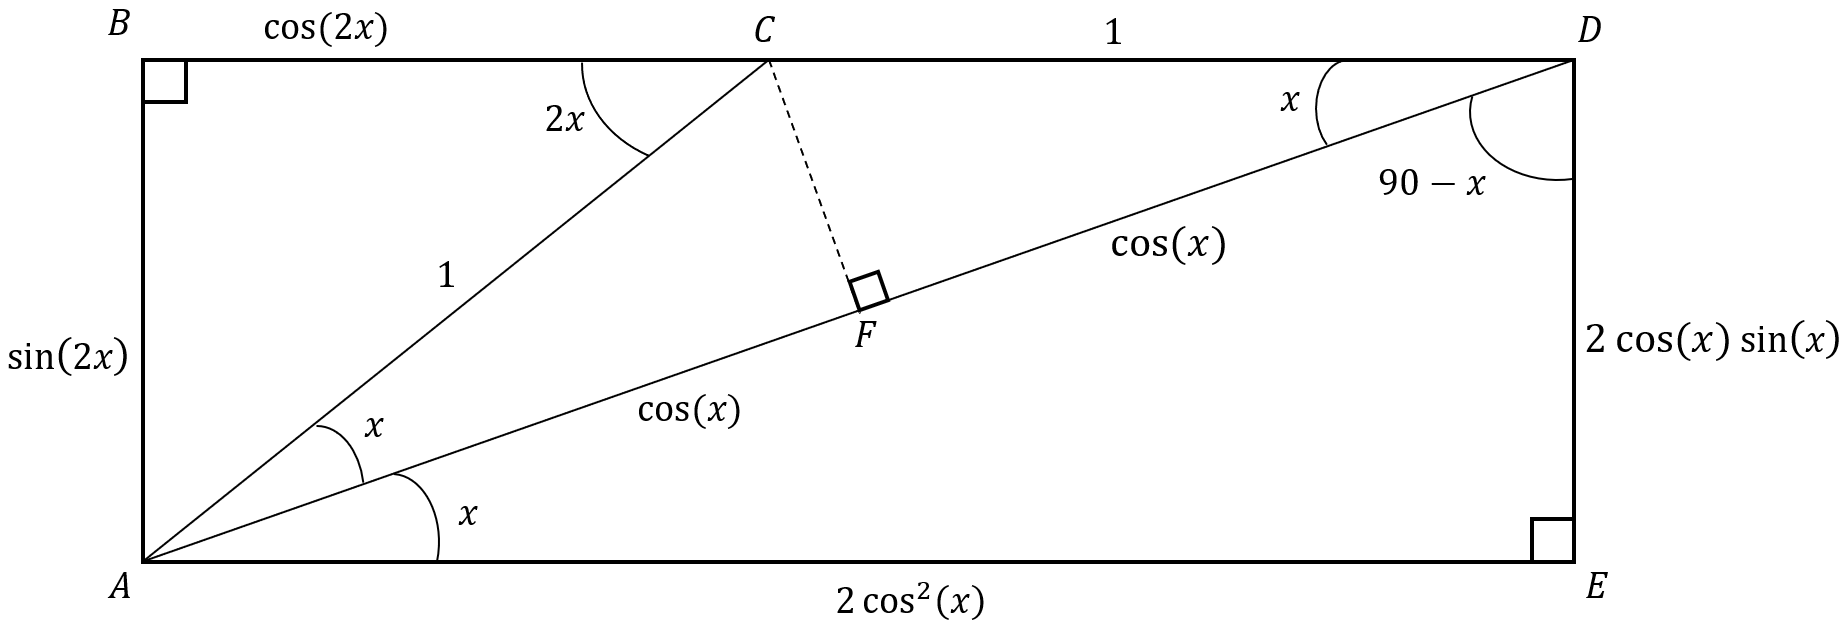
\includegraphics[width=\textwidth]{doubleangleformulae}}
\end{figure}
Define the rectangle $ABDE$ such that $D\hat{A}E=x$, and position $C$ along $BD$ such that $AC=CD=1$.
\begin{flalign*}
C\hat{D}A&=x & & \text{(alternate angles)} && \\
C\hat{A}D&=x & & \text{(isosceles triangle)} && \\
C\hat{A}E&=2x & & && \\
A\hat{C}B&=2x & & \text{(alternate angles)} && \\
AB&=\sin(2x) & & \text{(trigonometric relation)} && \\
BC&=\cos(2x) & & \text{(trigonometric relation)} && \\
AF&=FD=\cos(x) & & \text{($CF$ is a perpendicular bisector)} && \\
AD&=2\cos(x) & & AF+FD=AD && \\
AE&=2\cos(x)\times\cos(x)=2\cos^{2}(x) & & \text{(trigonometric relation)} && \\
DE&=2\cos(x)\sin(x) & & \text{trigonometric relation)} && \\
& & & && \\
AB&=DE & \Rightarrow &\sin(2x)=2\cos(x)\sin(x) && \\
BD&=AE & \Rightarrow &\cos(2x)=2\cos^{2}(x)-1 &&
\end{flalign*}

\begin{flalign*}
\frac{\sin(2x)}{\cos(2x)}&=\frac{2\cos(x)\sin(x)}{\cos^{2}(x)-\sin^{2}(x)} && \\
\tan(2x)&=\frac{2\cos(x)\sin(x)}{\cos^{2}(x)-\sin^{2}(x)} &=\frac{\frac{2\cos(x)\sin(x)}{cos^{2}(x)}}{\frac{\cos^{2}(x)-\sin^{2}(x)}{\cos^{2}(x)}} &=\frac{2\frac{\sin(x)}{\cos(x)}}{\frac{\cos^{2}(x)}{\cos^{2}(x)}-\frac{\sin^{2}(x)}{\cos^{2}(x)}} && \\
& && \\
\tan(2x)&=\frac{2\tan(x)}{1-\tan^{2}(x)}
\end{flalign*}

So, the \emph{double angle formulae} are as follows:
\begin{align*}
\cos(2\theta)&\equiv 
\begin{cases}
\cos^{2}(\theta)-\sin^{2}(\theta) \\
2\cos^{2}(\theta)-1 \\
1-2\sin^{2}(\theta)
\end{cases} \\
\sin(2\theta)&\equiv 2\sin(\theta)\cos(\theta) \\
\tan(2\theta)&\equiv \frac{2\tan(\theta)}{1-\tan^{2}(\theta)}
\end{align*}

These can be used as substitutions when integrating functions involving terms of $\cos^{2}$ and $\sin^{2}$
\begin{itemize}
\item[Note:] The double angle formulae can be obtained from the \emph{compound angle formulae} (see section \ref{compoundangleformulae}) by setting $A=B$, which are given in the formula booklet.
\end{itemize}
\vspace{0.2cm}


\subsection{Compound angle formulae}
\label{compoundangleformulae}
\begin{itemize}
\item A Level M Year 2 \hspace{1cm} \phantom{ AS / } Pages 165 -- 167
\end{itemize} \par
A geometric derivation for the compound angle formulae for $\sin$, $\cos$, and $\tan$ is provided here. A matrix method can also be used, which extends the validity of these formulae to all $\theta$, which is also briefly demonstrated. While the matrix method is a quicker way of deriving them should you need to, they are also given in the formula booklet.

\subsubsection*{Geometric method}
\begin{figure}[H]
\centering
\scalebox{.95}{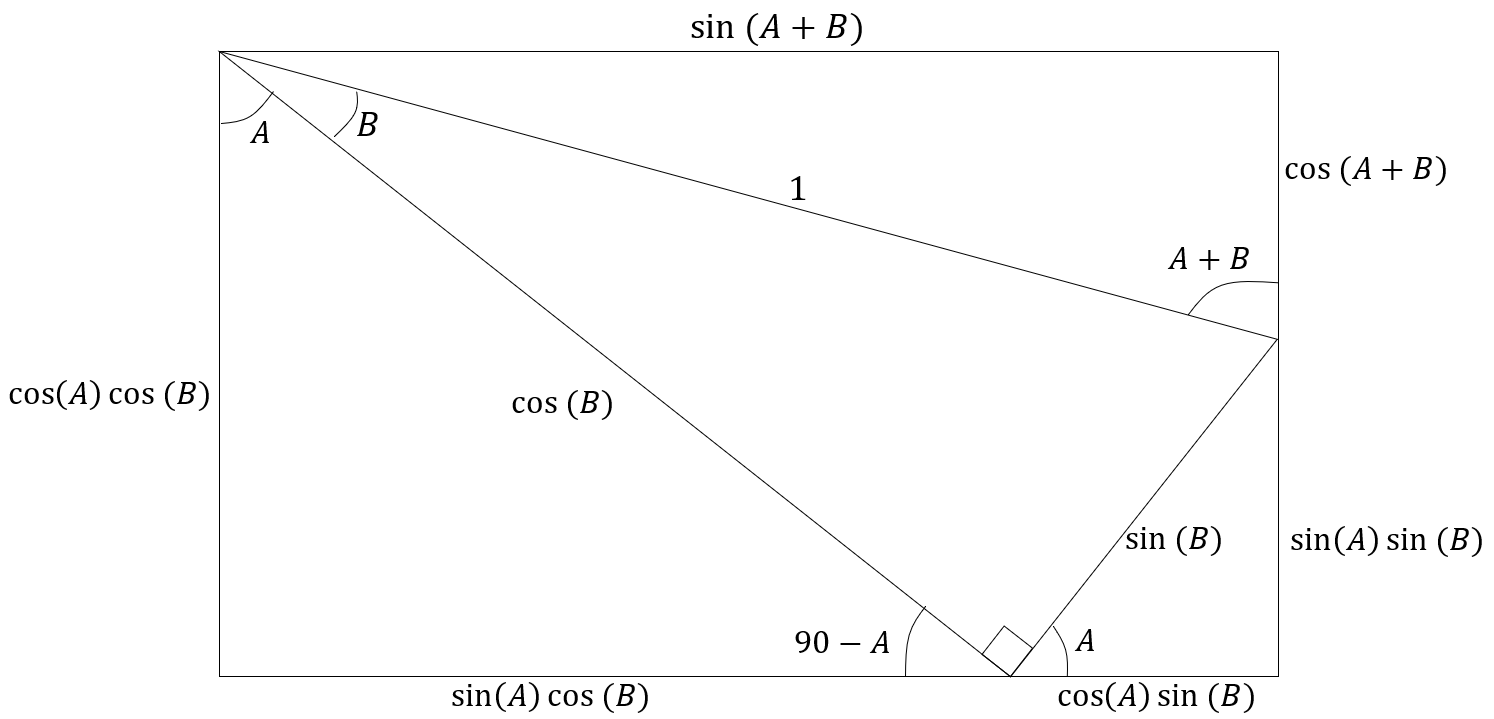
\includegraphics[width=\textwidth]{compoundangleformulae1}}
\end{figure}
The figure has all the side lengths marked on using simple trigonometric relations, and by rescaling such that a particular side has length 1 with two of the angles of size $A$ and $B$ (marked), the compound angle formulae follow quite straightforwardly:
\begin{align*}
\sin(A+B)&=\sin(A)\cos(B)+\cos(A)\sin(B) \\
\cos(A+B)&=\cos(A)\cos(B)-\sin(A)\sin(B) \\
\tan(A+B)&=\frac{\tan(a)+\tan(B)}{1-\tan(A)\tan(B)}
\end{align*}

By replacing $B$ with $-B$, we get the angle difference formulae. This can be deduced using the even / odd nature of $\sin$ and $\cos$.
\begin{align*}
\sin(A-B)&=\sin(A)\cos(B)-\cos(A)\sin(B) \\
\cos(A-B)&=\cos(A)\cos(B)+\sin(A)\sin(B) \\
\tan(A-B)&=\frac{\tan(a)-\tan(B)}{1+\tan(A)\tan(B)}
\end{align*}\par
\begin{itemize}
\item[Note:] This is only valid for positive angles less than $90^{\circ}$ / $\frac{\pi}{2}$ rad.
\end{itemize}

\subsubsection*{Matrix method}
The matrix $M=\begin{pmatrix} \cos(\theta) & -\sin(\theta) \\ \sin(\theta) & \cos(\theta) \end{pmatrix}$ represents a rotation of angle $\theta^{\circ}$ anticlockwise.
\begin{multline*}
\begin{pmatrix} \cos(\theta) & -\sin(\theta) \\ \sin(\theta) & \cos(\theta) \end{pmatrix} \begin{pmatrix} \cos(\phi) & -\sin(\phi) \\ \sin(\phi) & \cos(\phi) \end{pmatrix} \\ =\begin{pmatrix} \cos(\theta)\cos(\phi)-\sin(\theta)\sin(\phi) & -\left( \sin(\theta)\cos(\phi)-\cos(\theta)\sin(\phi) \right) \\ \sin(\theta)\cos(\phi)-\cos(\theta)\sin(\phi) & \cos(\theta)\cos(\phi)-\sin(\theta)\sin(\phi) \end{pmatrix}
\end{multline*}

Combined, this shows a rotation of an angle $\theta^{\circ}$ followed by a rotation of an angle $\phi^{\circ}$. Alternatively, this could be achieved by a single matrix representing a rotation of $(\theta+\phi)^{\circ}$ with elements:
\begin{equation*}
\begin{pmatrix} \cos(\theta+\phi) & -\sin(\theta+\phi) \\ \sin(\theta+\phi) & \cos(\theta+\phi) \end{pmatrix}
\end{equation*}
The compound angle formulae can then be trivially read off by matching the matrix elements. This also extends the validity to any angles $\theta$ and $\phi$.
\vspace{0.5cm}


\subsection{Harmonic Form -- superposition of waves of the same frequency}
\begin{itemize}
\item A Level M Year 2 \hspace{1cm} \phantom{ AS / } Pages 173 -- 178
\end{itemize} \par
This is a method that superimposes two (or more) waves which are of the \underline{same frequency}. It employs the compound angle formulae (see section \ref{compoundangleformulae}) to combine the two waves into a singular wave with some amplitude and phase shift. See below for a couple of worked examples.
\small
\begin{flalign*}
& && \\
\frac{\sqrt{3}}{2}\sin(x)-\frac{1}{2}\cos(x)&=\sin(x)\cos\left(\frac{\pi}{6}\right)-\cos(x)\sin\left(\frac{\pi}{6}\right) && \\
&=\sin\left(x-\frac{\pi}{6}\right) && \\
& && \\
\sin(x)+\cos(x)&=\sqrt{2}\left( \frac{1}{\sqrt{2}}\sin(x) + \frac{1}{\sqrt{2}}\cos(x) \right) && \\
&=\sqrt{2}\left(\cos\left(\frac{\pi}{4}\right)\sin(x)+\sin\left(\frac{\pi}{4}\right)\cos(x)\right) && \\
&=\sqrt{2}\cos\left(x-\frac{\pi}{4}\right) &&
\end{flalign*}
\normalsize

These are `nice' examples, where the phase shift is an easy factor to compute. More often than not, the examples will not be as trivial. A slightly more general way of answering these questions follows. Some questions may ask specifically for the combined wave to be a $\sin$ or $\cos$ wave with a phase shift. This can be done very simply by choosing the right form of $\sin(A\pm B)$ or $\cos(A\pm B)$. The choice of $+$ or $-$ is completely arbitrary, but a considered choice can make life much simpler. \newline \par

Take for example the expression $3\cos(x)-4\sin(x)$. Suppose we want to write this as a single cosine wave. This can be done as follows:
\begin{flalign*}
3\cos(x)-4\sin(x) &= R\cos(x+\alpha) && \\
&=R\cos(\alpha)\cos(x)-R\sin(\alpha)\sin(x) &&
\end{flalign*}
Collecting terms of $\cos(x)$ and $\sin(x)$ alike;
\begin{flalign*}
3\cos(x)&=R\cos(\alpha)\cos(x) & 3=R\cos(\alpha) && \\
4\sin(x)&=R\sin(\alpha)\sin(x) & 4=R\sin(\alpha) &&
\end{flalign*}
\begin{flalign*}
\frac{R\sin(\alpha)}{R\cos(\alpha)}&=\frac{4}{3} & R^{2}\sin^{2}(\alpha)&=16 && \\
\tan(\alpha)&=\frac{4}{3} & R^{2}\cos^{2}(\alpha)&=9 && \\
\alpha&=\arctan\left(\frac{4}{3}\right)+n\pi & R^{2}\left( \sin^{2}(\alpha)+\cos^{2}(\alpha) \right)&=25 && \\
& & R^{2}&= 25 \hspace{0.25cm} \Rightarrow \hspace{0.25cm} R=5 &&
\end{flalign*}
\footnotesize{Take principle value of $\alpha$ provided correct choice of $+$/$-$ earlier, so that $0\leq\alpha\leq\frac{\pi}{2}$} \newline \par
\normalsize

Thus;
\begin{equation*}
3\cos(x)-4\sin(x)=5\cos\left( x+\arctan\left(\frac{4}{3}\right) \right)
\end{equation*}\par

Suppose we wanted this in the form of $R\cos(x\textcolor{red}{-}\alpha)$. The expansion has the difference of a `$+$' instead of a `$-$' between the two terms involving $\cos(x)$ and $\sin(x)$. \par
\begin{flalign*}
3\cos(x)-4\sin(x) &= R\cos(x\textcolor{red}{-}\alpha) && \\
&=R\cos(\alpha)\cos(x)\textcolor{red}{+}R\sin(\alpha)\sin(x) &&
\end{flalign*}
Again, collecting terms of $\cos(x)$ and $\sin(x)$ alike;
\begin{flalign*}
3\cos(x)&=R\cos(\alpha)\cos(x) & 3=R\cos(\alpha) && \\
\textcolor{red}{-}4\sin(x)&=R\sin(\alpha)\sin(x) & \textcolor{red}{-}4=R\sin(\alpha) &&
\end{flalign*}
\begin{flalign*}
\frac{R\sin(\alpha)}{R\cos(\alpha)}&=\frac{\textcolor{red}{-}4}{3} & R^{2}\sin^{2}(\alpha)&=16 && \\
\tan(\alpha)&=\frac{\textcolor{red}{-}4}{3} & R^{2}\cos^{2}(\alpha)&=9 && \\
\alpha&=\arctan\left(\frac{\textcolor{red}{-}4}{3}\right)+n\pi & R^{2}\left( \sin^{2}(\alpha)+\cos^{2}(\alpha) \right)&=25 && \\
& & R^{2}&= 25 \hspace{0.25cm} \Rightarrow \hspace{0.25cm} R=5 &&
\end{flalign*}

Thus;
\begin{align*}
3\cos(x)-4\sin(x)&=5\cos\left( x\textcolor{red}{-}\arctan\left(\frac{\textcolor{red}{-}4}{3}\right) \right) \\
&=5\cos\left( x\textcolor{red}{+}\arctan\left(\frac{4}{3}\right) \right)
\end{align*}
as expected. \newline \par
Of course, we could also have chosen to write this in terms of a sine wave, again with free choice of whether it is $+\alpha$ or $-\alpha$ in the argument.
\vspace{0.5cm}


\subsection{The inverse trigonometric functions}
\begin{itemize}
\item A Level M Year 2 \hspace{1cm} \phantom{ AS / } Pages 134 -- 139
\end{itemize} \par
As stated in the section on inverse functions (section \ref{inversefunctions}) the graph of the inverse function can be obtained by a reflection in the line $y=x$. However, if the domains and codomains are left unrestricted, then the inverse function will be multi-valued for all of $\sin$, $\cos$, and $\tan$, which is not allowed for a function if it is to be properly defined (see section \ref{formalisingfunctions}). The domains and codomains for the three trigonometric functions are listed below, with the inverse functions swapping the restricted domain and codomain.


\begin{center}
\small
\begin{tblr}{|[.75pt]|l||c|c|c||[.75pt]}
\hline[1.25pt]
 & $\sin$ & $\cos$ & $\tan$ \\ \hline[.75pt]
Unrestricted & $\mathbb{R}\rightarrow[-1,1]$ & $\mathbb{R}\rightarrow[-1,1]$ & $\mathbb{R}\setminus\left\{ \pm\frac{\pi}{2},\pm\frac{3\pi}{2},\dots \right\} \rightarrow \mathbb{R}$ \\ \hline
Restricted & $\left[ -\frac{\pi}{2},\frac{\pi}{2} \right]\rightarrow[-1,1]$ & $\left[ 0,\pi \right]\rightarrow[-1,1]$ & $\left( -\frac{\pi}{2},\frac{\pi}{2} \right) \rightarrow \mathbb{R}$ \\ \hline
Inverse &  $\left[ -1,1 \right]\rightarrow[-\frac{\pi}{2},\frac{\pi}{2}]$ & $\left[ -1,1 \right]\rightarrow[0,\pi]$ & $\mathbb{R} \rightarrow \left( -\frac{\pi}{2},\frac{\pi}{2} \right)$ \\ \hline[1pt]
\end{tblr}
\normalsize
\end{center}

\vspace{0.5cm}


\subsection{Derivatives of sine and cosine}
\begin{itemize}
\item A Level M Year 2 \hspace{1cm} \phantom{ AS / } Pages 185 -- 195
\end{itemize} \par
The derivatives of trigonometric functions are closely linked and are set out below. A proof follows, though there are other ways of proving this.
\begin{center}
\begin{tblr}{|[.75pt]|c|c||[.75pt]}
\hline[1.25pt]
$f(x)$ & $\frac{\mathrm{d}}{\mathrm{d}x}\left[ f(x) \right]$ \\ \hline[.75pt]
$\sin(x)$ & $\cos(x)$ \\ \hline
$\cos(x)$ & $-\sin(x)$ \\ \hline[1pt]
\end{tblr}
\end{center}
Proof:
\begin{figure}[H]
\centering
\scalebox{.4}{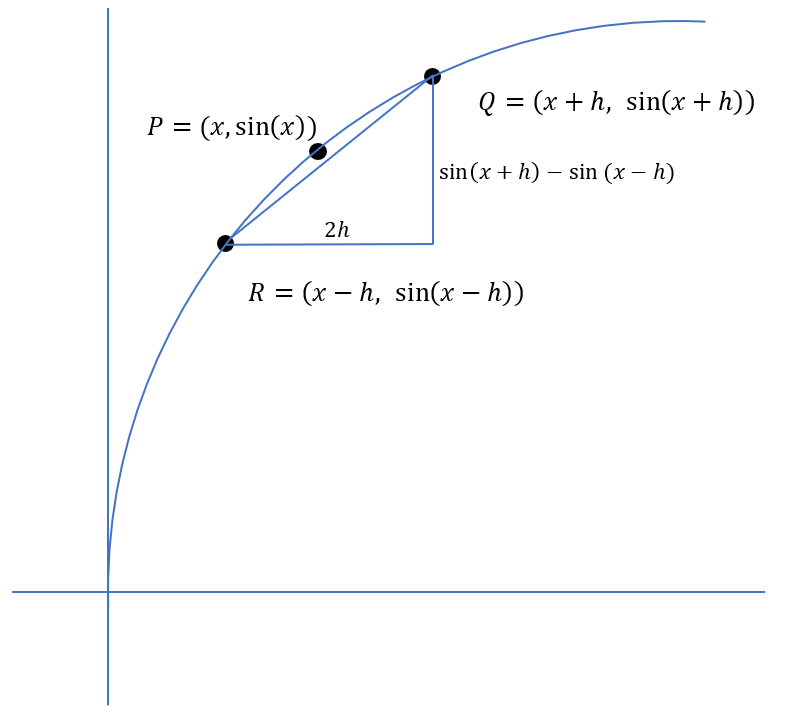
\includegraphics[width=\textwidth]{sinederivation1}}
\end{figure}
From first principles, we can say that:
\begin{equation*}
\frac{\mathrm{d}}{\mathrm{d}x}\left[\sin(x)\right]=\lim_{h\to0}\left[\frac{\sin(x+h)-\sin(x-h)}{2h}\right]
\end{equation*}
and using compound angle formulae (section \ref{compoundangleformulae}), we have:
\begin{equation*}
\sin(x+h)-\sin(x-h)=2\cos(x)\sin(h)
\end{equation*}
Thus:
\begin{equation*}
\frac{\mathrm{d}}{\mathrm{d}x}\left[\sin(x)\right]=\lim_{h\to0}\left[\frac{2\cos(x)\sin(h)}{2h}\right]=\lim_{h\to0}\left[\frac{\cos(x)\sin(h)}{h}\right]
\end{equation*}
\begin{figure}[H]
\centering
\scalebox{.95}{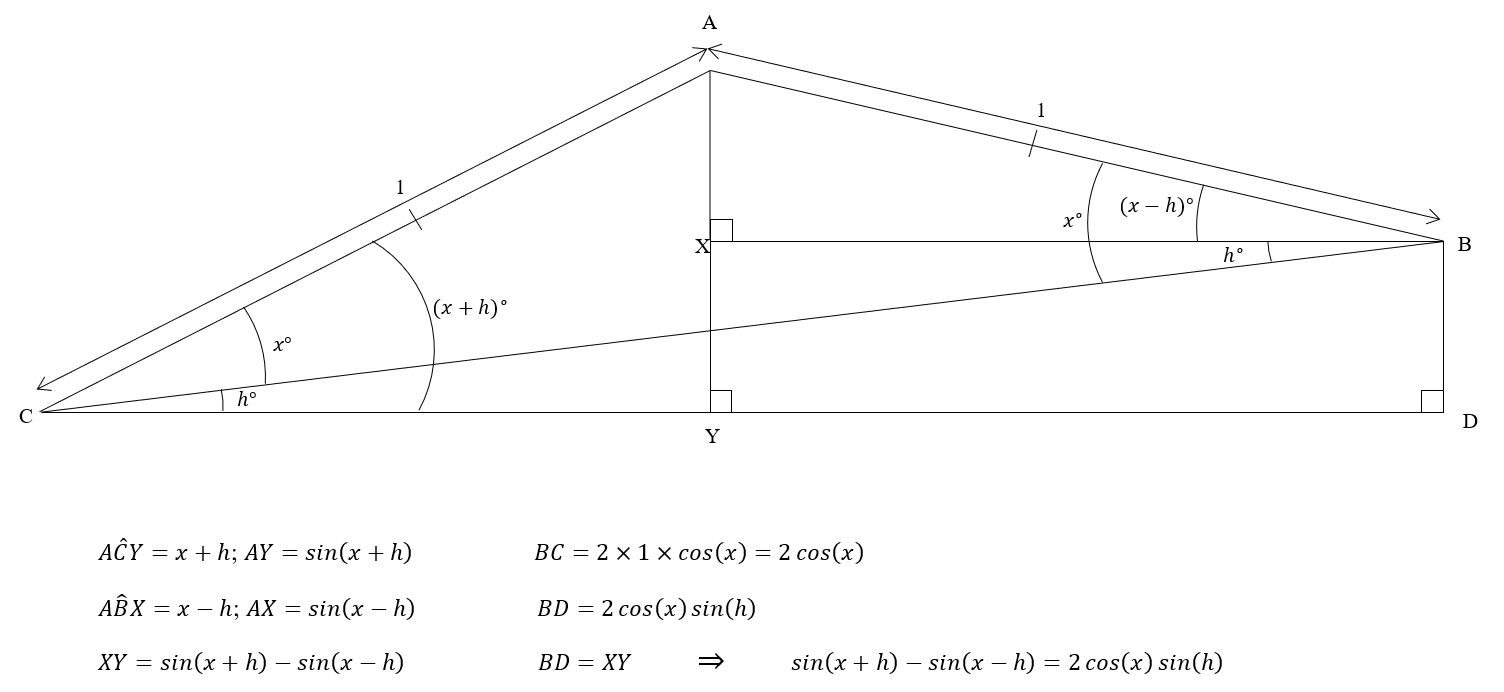
\includegraphics[width=\textwidth]{sinederivation2}}
\end{figure}
and since $\cos(x)$ is fixed:
\begin{equation*}
\lim_{h\to0}\left[\frac{\cos(x)\sin(h)}{h} \right]=\cos(x)\times\lim_{h\to0}\left[ \frac{\sin(h)}{h}\right]
\end{equation*}
Again requiring radians to be used, this limit evaluates to 1 when working in radians\footnote{This limit evaluates to $\frac{\pi}{180}$ when working in degrees}, so we recover:
\begin{equation*}
\frac{\mathrm{d}}{\mathrm{d}x}\left[ \sin(x) \right]=\cos(x)
\end{equation*}
To then find the derivative of $\cos(x)$, we can use a trick involving the chain rule. $\cos(x)$ can be written as a composite function, with
\begin{equation*}
\cos(x)=\sin\left( \frac{\pi}{2}-x \right)
\end{equation*}
Then taking the derivative of both sides, and applying the chain rule;
\begin{align*}
\frac{\mathrm{d}}{\mathrm{d}x}\left[ \cos(x) \right] &= \frac{\mathrm{d}}{\mathrm{d}x}\left[ \sin\left( \frac{\pi}{2}-x \right) \right] \\
&=\cos\left( \frac{\pi}{2}-x \right)\cdot\frac{\mathrm{d}}{\mathrm{d}x}\left[ \frac{\pi}{2}-x \right] \\
&=-\cos\left( \frac{\pi}{2}-x \right) \\
&=-\sin(x)
\end{align*}
Therefore;
\begin{equation*}
\frac{\mathrm{d}}{\mathrm{d}x}\left[ \cos(x) \right]=-\sin(x)
\end{equation*}
\vspace{0.5cm}


\subsection{Derivatives of standard and reciprocal trigonometric functions}
\begin{itemize}
\item A Level M Year 2 \hspace{1cm} \phantom{ AS / } Pages 185 -- 195
\end{itemize} \par

Here is a list of the derivatives of standard and reciprocal trigonometric functions. The reciprocal functions can be obtained by applying the quotient rule (section \ref{quotientrule}).

\begin{center}
\begin{tblr}{|[.75pt]|c|c||[.75pt]}
\hline[1.25pt]
$f(x)$ & $\frac{\mathrm{d}}{\mathrm{d}x}\left[ f(x) \right]$ \\ \hline[.75pt]
$\sin(x)$ & $\cos(x)$ \\ \hline
$\cos(x)$ & $-\sin(x)$ \\ \hline
$\tan(x)$ & $\sec^{2}(x)$ \\ \hline
$\cosec(x)$ & $-\cosec(x)\cot(x)$ \\ \hline
$\sec(x)$ & $\sec(x)\tan(x)$ \\ \hline
$\cot(x)$ & $-\cosec^{2}(x)$ \\ \hline[1pt]
\end{tblr}
\end{center}

\vspace{0.5cm}


\subsection{Derivatives of the inverse trigonometric functions}
\label{inversetrigderivatives}
\begin{itemize}
\item A Level FM Year 2 \hspace{1cm} \phantom{AS /} Pages 152 -- 157
\end{itemize} \par
The derivatives of inverse trigonometric functions can be found using implicit differentiation (see section \ref{implicitdifferentiation}). A brief demonstration for the derivatives of $\arccos$, $\arcsin$, and $\arctan$ follow. 
\subsubsection*{arcsin}
\vspace{-0.8cm}
\begin{flalign*}
y&=\arcsin(x) && \\
x&=\sin(y) && \\
1&=\cos(y)\frac{\mathrm{d}y}{\mathrm{d}x} && \\
\frac{\mathrm{d}y}{\mathrm{d}x}&=\frac{1}{\cos(y)}=\frac{1}{\pm\sqrt{1-\sin^{2}(y)}}=\frac{1}{\pm\sqrt{1-x^{2}}} && \\
&\text{\small{ Gradient always positive, so: }} && \\
\frac{\mathrm{d}y}{\mathrm{d}x}&=\frac{1}{\sqrt{1-x^{2}}} && \\
\end{flalign*}
\subsubsection*{arccos}
\vspace{-0.8cm}
\begin{flalign*}
y&=\arccos(x) && \\
x&=\cos(y) && \\
1&=-\sin(y)\frac{\mathrm{d}y}{\mathrm{d}x} && \\
\frac{\mathrm{d}y}{\mathrm{d}x}&=\frac{-1}{\sin(y)}=\frac{-1}{\pm\sqrt{1-\cos^{2}(y)}}=\frac{1}{\mp\sqrt{1-x^{2}}} && \\
&\text{\small{ Gradient always negative, so: }} && \\
\frac{\mathrm{d}y}{\mathrm{d}x}&=-\frac{1}{\sqrt{1-x^{2}}} && \\
\end{flalign*}
\subsubsection*{arctan}
\vspace{-0.8cm}
\begin{flalign*}
y&=\arctan(x) && \\
x&=\tan(y) && \\
1&=\sec^{2}(y)\frac{\mathrm{d}y}{\mathrm{d}x} && \\
\frac{\mathrm{d}y}{\mathrm{d}x}&=\frac{1}{\sec^{2}(y)}=\frac{1}{1+\tan^{2}(y)}=\frac{1}{1+x^{2}} &&
\end{flalign*}

\subsection{Integrals using trigonometric identities}
\begin{itemize}
\item A Level M Year 2 \hspace{1cm} \phantom{ AS / } Pages 234 -- 239
\end{itemize}
Integrals containing powers of trigonometric functions can be dealt with by using identities involving these functions. A general integral involving powers of sines and cosines\footnote{The other Pythagorean identities can be used for integrals involving powers of the tangent and secant, or powers of the cotangent and cosecant} has the form
\begin{equation*}
\int \sin^{m}(x)\cos^{n}(x)\,\mathrm{d}x
\end{equation*}
and has three main cases:
\begin{itemize}
\item[Case 1:] Power of sine is odd and positive
\item[] For an odd powered sine term, take off a $\sin(x)$ and put it at the end
\begin{equation*}
\int \sin^{2n+1}(x)\cos^{m}(x)\,\mathrm{d}x=\int\sin^{2n}(x)\cos^{m}(x)\times\sin(x)\,\mathrm{d}x
\end{equation*}
Then, turn every remaining even power of sine into cosines using a trigonometric identity.
\begin{equation*}
\int \sin^{2n}(x)\cos^{m}(x)\times\sin(x)\,\mathrm{d}x=\int \left( 1-\cos^{2}(x) \right)^{n}\cos^{m}(x)\times\sin(x)\,\mathrm{d}x
\end{equation*}
Now, we can simply expand out the brackets, and since the remaining sine term can be treated as the result of a chain rule, the integral can be done by inspection, as it is essentially a polynomial in $\cos(x)$.
\newpage
\item[Case 2:] Power of cosine is odd and positive
\item[] This is essentially the same as for Case 1. For an odd powered cosine term, take off a $\cos(x)$ and put it at the end
\begin{equation*}
\int \sin^{n}(x)\cos^{2m+1}(x)\,\mathrm{d}x=\int\sin^{n}(x)\cos^{2m}(x)\times\cos(x)\,\mathrm{d}x
\end{equation*}
Then, turn every remaining even power of cosine into sines using a trigonometric identity.
\begin{equation*}
\int \sin^{n}(x)\cos^{2m}(x)\times\cos(x)\,\mathrm{d}x=\int \sin^{n}(x)\left( 1-\sin^{2}(x) \right)^{m}\times\cos(x)\,\mathrm{d}x
\end{equation*}
Now, we can simply expand out the brackets, and since the remaining cosine term can be treated as the result of a chain rule, the integral can be done by inspection, as it is essentially a polynomial in $\sin(x)$.
\item[Case 3:] Powers of both sine and cosine are even and positive
\item[] In this case, we need to use half-angle trigonometric identities to convert the integrand into \emph{odd} powers of cosines.
\begin{align*}
\sin^{2}(x)&\frac{1-\cos(2x)}{2} \\
\cos^{2}(x)&=\frac{1+\cos(2x)}{2}
\end{align*}
So, for example,
\begin{align*}
\int\sin^{2}(x)\cos^{2}(x)\,\mathrm{d}x&=\int\left[ \sin^{2}(x)\frac{1-\cos(2x)}{2} \right]\left[ \cos^{2}(x)\frac{1+\cos(2x)}{2} \right]\,\mathrm{d}x \\
&=\frac{1}{4}\int 1-\cos^{2}(2x)\,\mathrm{d}x \\
&=\frac{1}{4}\int 1-\frac{1+\cos(4x)}{2}\,\mathrm{d}x \\
&=\frac{1}{8}\int 2-1-\cos(4x)\,\mathrm{d}x \\
&=\frac{1}{8}\int 1-\cos(4x)\,\mathrm{d}x \\
&=\frac{1}{8}x-\frac{1}{32}\sin(4x)+c
\end{align*}
\end{itemize}
\vspace{0.5cm}


\subsection{Integrals via inverse trigonometric functions: Standard results}
\begin{itemize}
\item A Level FM Year 2 \hspace{1cm} \phantom{AS /} Pages 152 -- 157
\end{itemize} \par
This is the origin of some of the integrals in the section on standard integrals, in section \ref{usefulintegrals}. They come from combining the results of the inverse trigonometric functions (section \ref{inversetrigderivatives}) with the chain rule (section \ref{chainrule}). Once again, these are in the formula booklet, so do not necessarily need to be memorised, but they should be recognised.

\begin{gather*}
\int\frac{1}{\sqrt{a^{2}-x^{2}}}\,\mathrm{d}x=\arcsin\left( \frac{x}{a} \right) + c \\
 \\
\int\frac{1}{a^{2}+x^{2}}\,\mathrm{d}x=\frac{1}{a}\arctan\left( \frac{x}{a} \right) + c \\
\end{gather*}

\vspace{0.5cm}

\end{document}